\documentclass[english, spanish, fleqn, 10pt]{article}
\usepackage[top = 2.5cm, bottom = 2cm, left = 2.5cm, right = 2.5cm]{geometry}
\usepackage{babel}
\usepackage[utf8]{inputenc}
\usepackage{amsthm, amsmath, amssymb, amsfonts, environ}
\usepackage{caption}
\usepackage{subcaption} % para las subfigures
\usepackage{mathrsfs}
\usepackage[colorlinks, urlcolor=blue,
pdfauthor={Aldo Berrios Valenzuela}]{hyperref}
\usepackage{fourier}
\usepackage{colortbl}
\usepackage{color}
\usepackage{graphicx}
\usepackage{enumitem}
%\renewcommand{\familydefault}{\sfdefault}
%\setlength{\parindent}{0pt}					%Espacio de sangria
\setlength{\parskip}{2mm}						%Interlinado entre párrafos
\usepackage{fancyhdr, blindtext}		%Paquete de encabezado
\usepackage{listings}
\usepackage[framemethod=tikz]{mdframed}

\definecolor{webred}{rgb}{0.75,0,0}
\definecolor{mblue}{rgb}{0.0705,0.345,0.7529}
\definecolor{newmblue}{HTML}{004D99}
\usepackage{longtable, colortbl, array}

\definecolor{superGreenNew}{HTML}{169F01}
\hypersetup{
	colorlinks   = true,
	citecolor    = superGreenNew
}


%==============================
%Modificador de Titulos de secciones, subsecciones, etc
\usepackage[explicit]{titlesec}

\titlespacing\subsubsection{0pt}{8pt plus 4pt minus 2pt}{0pt plus 2pt minus 2pt}


%==================================
%Diseno para insertar codigos de programacion
\definecolor{newGray}{HTML}{F8F8F8}
\definecolor{anotherGray}{HTML}{DDDFFF}
\lstdefinestyle{customc}{
	belowcaptionskip=1\baselineskip,
	breaklines=true,
	backgroundcolor=\color{newGray},
	frame=single,
	rulecolor=\color{anotherGray},
	xleftmargin=\parindent,
	language=bash,
	showstringspaces=false,
	basicstyle=\small\ttfamily,
	keywordstyle=\bfseries\color{green!40!black},
	commentstyle=\itshape\color{purple!40!black},
	identifierstyle=\color{black},
	stringstyle=\color{mblue},
	tabsize=2,
	literate={\ \ }{{\ }}1	
}
\lstset{style=customc}

%==================================
%Macros útiles
\newcommand{\comillas}[1]{``#1''}
\newcommand{\comentarioc}[1]{\texttt{\textcolor{webred}{/* #1 */}}}

\numberwithin{equation}{section}

%=================================
%comandos matemáticos personalizados de rápido acceso
\newcommand{\nparentesis}[1]{\left( #1 \right)}
\newcommand{\llaves}[1]{\left \{ #1 \right \}}
\newcommand{\nabsoluto}[1]{\left| #1 \right|}
\newcommand{\ncorchetes}[1]{\left[ #1 \right]}
%=================================

%cambia el espaciado entre el parrafo y antes del itemize
\setlist[itemize]{itemsep=1mm, topsep=0.5mm}
\setlist[enumerate]{itemsep=1mm, topsep=0.5mm}
%===========================

\theoremstyle{definition}
\newtheorem{teorema}{Teorema}[section]
\newtheorem{definition}{Definición}[section]
\newtheorem{beforeExample}{Ejemplo}[section]
\newtheorem{preposicion}{Preposición}[section]
\newtheorem{corolario}{Corolario}[teorema]

\captionsetup{justification=centering, margin=2.3cm}

\newenvironment{ejemplo}[1][]{\begin{beforeExample}[#1]\renewcommand{\qedsymbol}{$\blacksquare$}}{\qed\end{beforeExample}}

\captionsetup{justification=centering, margin=2.3cm}

% Para poder hacer "quote" con estilo github

\newenvironment{newquote}{\begin{mdframed}[topline=false,
		rightline=false, bottomline=false, linewidth=.3em,backgroundcolor=black!5, linecolor=black!60]\color{black!70}}{\end{mdframed}}
%================================


\usepackage{fancyhdr}

\pagestyle{fancy}
\lhead{INF221\quad Algoritmos y Complejidad}
\rhead{\textit{Ayudantía \#4\quad Algoritmos Voraces}}

\author{Aldo Berrios Valenzuela}
\title{INF221 -- Algoritmos y Complejidad\\[.4\baselineskip]Ayudantía \#4\\Algoritmos Voraces}


\usepackage{tikz,ifthen}
\usetikzlibrary{automata,positioning, babel}
\definecolor{navyblue}{RGB}{0,148,222}
\usetikzlibrary{fit}
\tikzset{shorten >=1pt,node distance=2cm,on grid, >=stealth, initial text=Inicio,
	every state/.style={ draw=navyblue!50,very thick,fill=navyblue!20, minimum size=6mm},
	bend angle=35, every loop/.style={looseness=13}}
\usetikzlibrary{calc}

\begin{document}
\maketitle
\section{Algoritmos Voraces}
Los algoritmos voraces encuentran una solución óptima, pero no necesariamente la \emph{más} óptima.

Para demostrar que un algoritmo es voraz tenemos que demostrar que:
\begin{itemize}
	\item \emph{Greedy Choice:} Para toda instancia\footnote{cuando hablamos de instancia es como decir un \comillas{momento} del problema} $P$, tal que hay una solución óptima que incluye $\hat p$; este es el primer elemento elegido.
	\begin{center}
		\comentarioc{Dibujo feo: un circulo deforme que contiene $P$ e inscrito a este tiene otro circulo $P'$. Leyenda: cada vez vamos escogiendo $\hat{p}$ tales que van achicando nuestro problema cada vez más.}
	\end{center}
	
	\item \emph{Inductive Structure:} Dada la elección de $\hat p$, queda un subproblema $P'$ (menor que el anterior), tal que si $\Pi'$ es solución óptima de $P'$, $\llaves{\hat p}\cup \Pi'$ es solución viable de $P$. \comentarioc{en el fondo, cada vez que sacamos un $\hat p$ para formar un nuevo $P'$, el resultado siempre será el mismo problema que tenemos que resolver}
	
	\item \emph{Optimal Subestructure:} Si $\Pi'$ es solución óptima para $P'$ y $\hat p$ es la elección voraz para $P$, entonces $\llaves{\hat p}\cup \Pi'$ es solución óptima para $P$.
\end{itemize}


\begin{ejemplo}[Árbol de Compensión de Hufmann]
	Es un algoritmo que utiliza \texttt{mp3} para comprimir datos. Nos dan una tabla con frecuencia y símbolo (Cuadro <>)
	\begin{table}[!h]
		\centering
		\begin{tabular}{c|c}
			Símbolo & Frecuencia\\
			\hline
			$A$&70 millones\\
			$B$&5 millones\\
			$C$&20 millones\\
			$D$&37 millones
		\end{tabular}
	\end{table}
	Y el arbol generado es:
	\begin{figure}[!h]
		\centering
		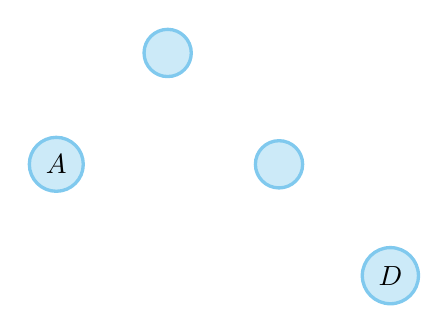
\begin{tikzpicture}
		\node [state] (0) {};
		\node [state, below left of = 0] (A) {$A$};
		\node [state, below right of = 0] (1) {};
		\node [state, below right of = 1] (D) {$D$};
		\end{tikzpicture}
	\end{figure}
	\begin{center}
		\comentarioc{Colocar arbol: valores más repetidos están más arriba}
	\end{center}
	Y luego el código de ese arbol está dado por el cuadro <>:
	\begin{table}
		\centering
		\begin{tabular}{c|c}
			Símbolo & Código\\
			\hline
			$A$&0\\
			$B$&100\\
			$C$&101\\
			$D$&11
		\end{tabular}
	\end{table}
	Luego, buscamos el costo del arbol:
	\begin{equation}
	\text{Cost}=\sum_{i=1}^nf_i\text{Depth}_i
	\end{equation}
	El árbol inicial es:
	\begin{center}
		\comentarioc{Arbol inicial}
	\end{center}
	En cada paso del algoritmo vamos sumando los menores para formar una expresión y llegar al grafo.
	\begin{align*}
	&\underbrace{C}_{20}, \underbrace{B}_{3}, \underbrace{D}_{37}, \underbrace{A}_{70}\\
	&\nparentesis{C+B}, D, A\\
	&\nparentesis{\nparentesis{C+B}+D}, A\\
	&\nparentesis{\nparentesis{\nparentesis{C+B}+D}+A}
	\end{align*}
	\begin{center}
		\comentarioc{Grafo: En el fondo, empezamos con los elementos que están dentro del mismo paréntesis. Por otro lado, todos aquellos que estén dentro del mismo paréntesis tienen al mismo padre.}
	\end{center}
	Ahora que sabe como funciona el árbol de compensación de Hufmann, demuestre que es óptimo.
\end{ejemplo}

\begin{proof}
	Demostramos cada uno de los puntos de algoritmo voraz:
	\begin{itemize}
		\item \emph{Greedy choice:}
		
		$C$ y $B$ son la mejor opción para el nivel más bajo. Opción:
		\begin{equation*}
		x\cdot 1+y\cdot 2+\underbrace{23}_{C+B}\cdot 3\qquad\comentarioc{1, 2, y 3 representan el nivel en el arbol}
		\end{equation*}
		
		\item \emph{Inductive structure:}
		
		\comentarioc{Explicar el tema de juntar los nodos, y ver que el problema que nos queda será el mismo que teníamos inicialmente, pero reducido. Si continuamos haciendo esta jugarreta siempre tendremos el mismo problema. Por lo tanto, cumple con la estructura óptima.}
		
		\item \emph{Optimal Subestructure:}
		
	\end{itemize}
\end{proof}

\begin{ejemplo}[Algoritmo de Kruskal]
	Genera un arbol recubridor mínimo:
	\begin{center}
		\comentarioc{colocar ambos grafos: original y recubridor mínimo}
	\end{center}
	Demuestre que es óptimo.
\end{ejemplo}
\begin{proof}
	Demostramos cada uno de los puntos de algoritmo voraz:
	\begin{itemize}
		\item \emph{Greedy choice:}
	\end{itemize}
\end{proof}



\end{document}